\documentclass[11pt]{article}

% ==== Paquetes ====
\usepackage[utf8]{inputenc}
\usepackage[spanish]{babel}
\usepackage[T1]{fontenc}
\usepackage{amsmath, amssymb, amsfonts, siunitx}
\usepackage{graphicx}
\usepackage{caption}
\usepackage{subcaption}
\usepackage{tikz}
\usepackage{geometry}
\usepackage{float}
\usepackage{hyperref}
\usepackage{minted}
\usepackage{mdframed}
\usepackage{pdfpages}

\usemintedstyle{perldoc}
\geometry{margin=2.5cm}

% ==== Datos de la tarea ====
\title{IEE3584 - Comunicaciones inalámbricas \\
Tarea 12}
\author{Nicolás Seguel}
\date{Noviembre 2025}

\begin{document}
\maketitle

\section*{Problema 29}

\subsection*{(1) Generación de símbolos QPSK}

Se generaron símbolos QPSK independientes y equiprobables para dos antenas transmisoras, construyendo la matriz:
\[
\mathbf{S} \in \mathbb{C}^{2 \times N_s}, \qquad S_{ij} \in \{\tfrac{1}{\sqrt{2}}(\pm1 \pm j)\}.
\]
Cada símbolo tiene energía unitaria, por lo que la energía total transmitida por instante se fija a $E_s = 2E_{\text{sym}}$.  
El código siguiente genera la matriz $\mathbf{S}$ y grafica las dos realizaciones de los símbolos generados para ambas antenas transmisoras.

\begin{minted}{python3}
# -----------------------
# 1) Generar S (QPSK)
# -----------------------
def gen_S_qpsk(seed: int, Ns: int = 1000, Es: float = 1.0) -> np.ndarray:
    """
    Genera matriz S de símbolos QPSK iid de forma (2, Ns).

    Parámetros
    ----------
    seed : int
        Semilla para RNG (reproducible).
    Ns : int
        Número de columnas (número de bloques).

    Retorna
    -------
    S : ndarray (2, Ns)
        Matriz de símbolos complejos QPSK.
    """
    rng = np.random.default_rng(seed)
    # QPSK: puntos (±1 ± j)/sqrt(2) -> energía unitaria por símbolo
    bits_i = rng.integers(0, 2, size=(2, Ns))
    bits_q = rng.integers(0, 2, size=(2, Ns))
    # map: 0 -> +1, 1 -> -1
    a = 1 - 2*bits_i
    b = 1 - 2*bits_q
    S = (a + 1j*b) / np.sqrt(2) * Es   # energía por símbolo = 1
    return S
\end{minted}

\begin{figure}[H]
    \centering
    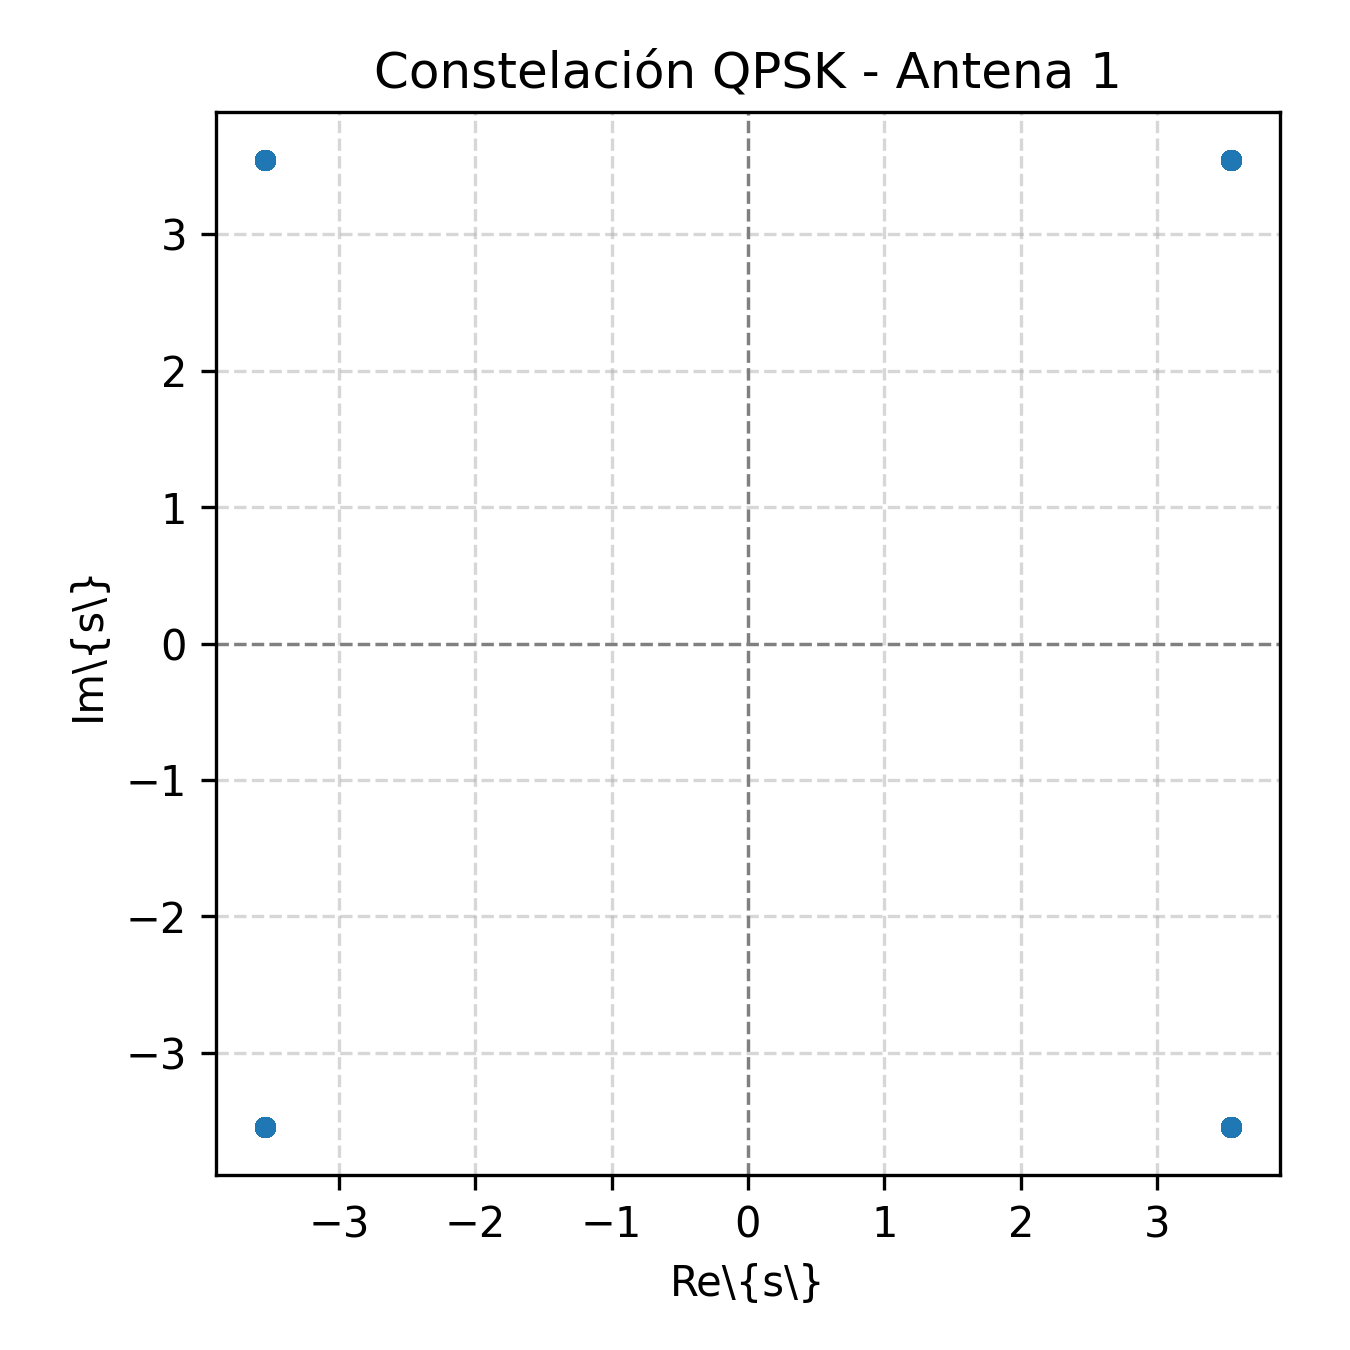
\includegraphics[width=0.48\textwidth]{figs/problema29_constellation_antenna1.png}
    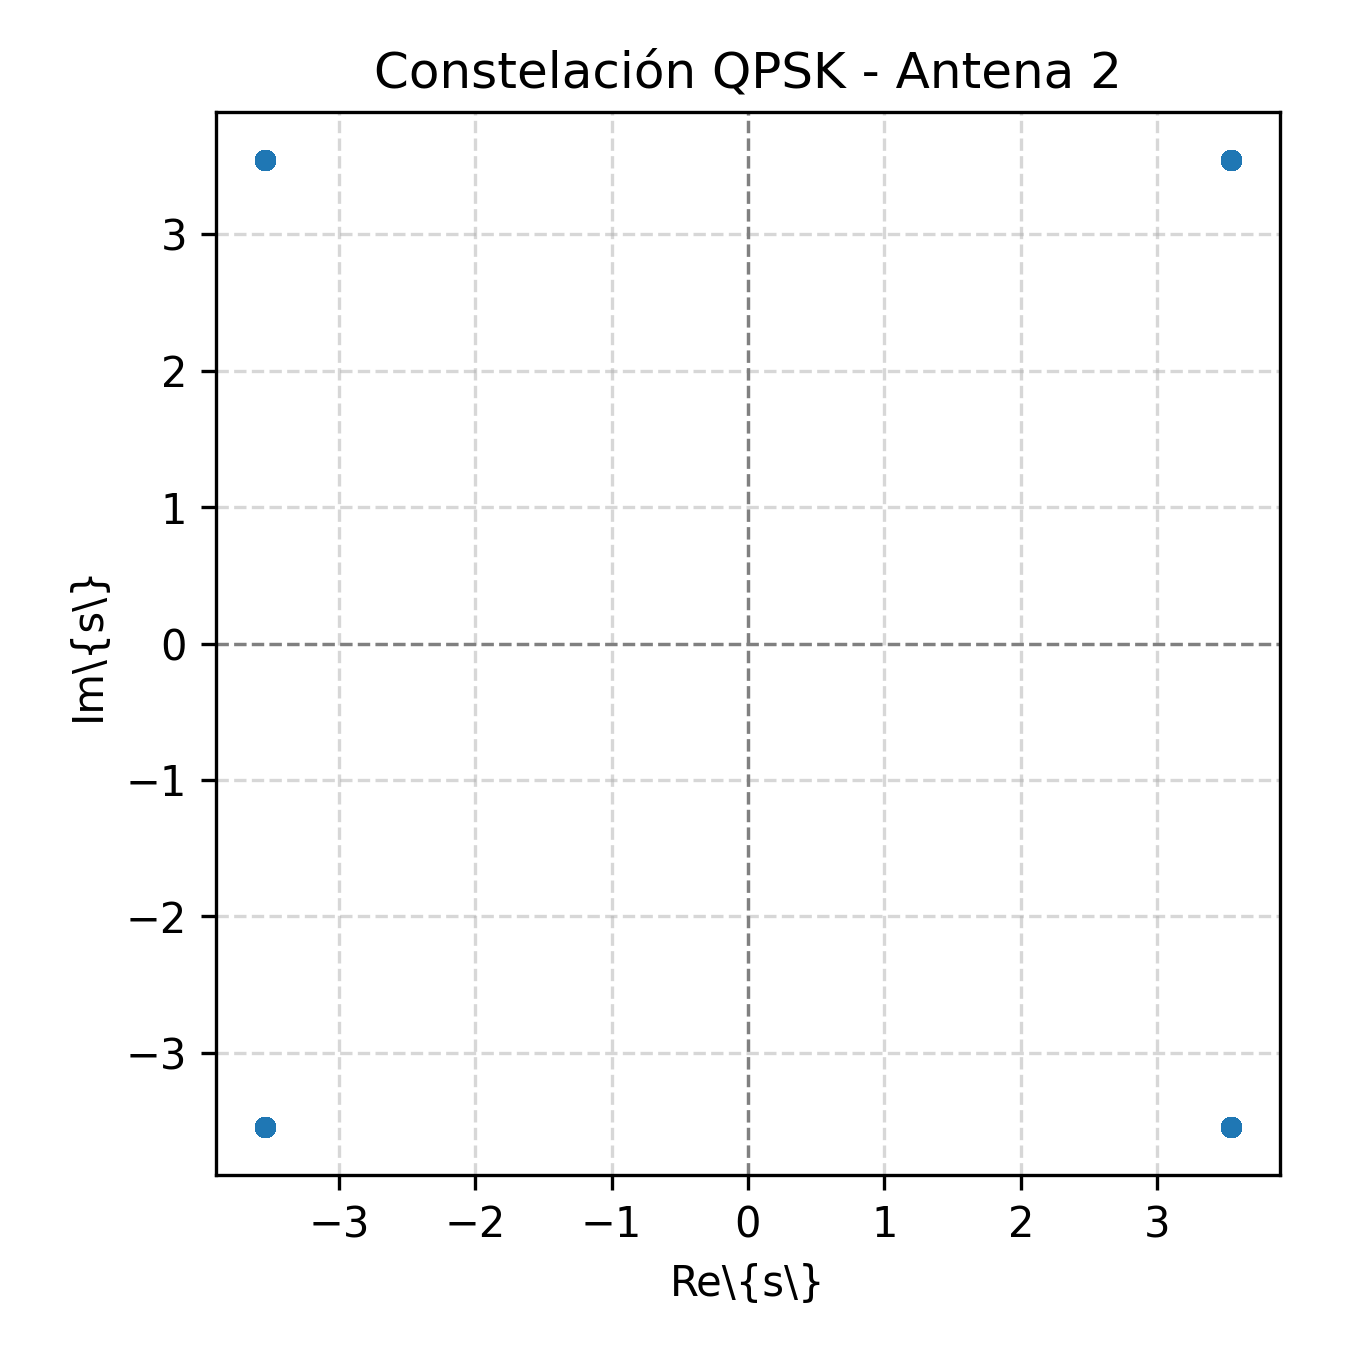
\includegraphics[width=0.48\textwidth]{figs/problema29_constellation_antenna2.png}
    \caption{Constelaciones QPSK generadas para las dos antenas transmisoras.}
\end{figure}

\subsection*{(2) Codificación Alamouti}

El esquema de Alamouti agrupa los símbolos $s_1, s_2$ en bloques de tiempo-espacio (STB):
\[
\mathbf{X}_n =
\begin{bmatrix}
s_1 & -s_2^* \\
s_2 &  s_1^*
\end{bmatrix},
\]
resultando en una matriz global $\mathbf{X}$ de dimensión $2\times 2N_s$.

\begin{minted}{python3}
# -----------------------
# 2) Codificador Alamouti
# -----------------------
def alamouti_encode(S: np.ndarray)-> np.ndarray:
    """
    Codifica la matriz S (2 x Ns) usando el esquema Alamouti por bloque.
    Cada columna de S: [s1; s2] se transforma en un bloque 2x2:
        [ s1   -conj(s2) ]
        [ s2    conj(s1) ]
    Concatenando sobre Ns obtenemos X de tamaño (2, 2*Ns).

    Parámetros
    ----------
    S : ndarray (2, Ns)

    Retorna
    -------
    X : ndarray (2, 2*Ns)
    """
    if S.ndim != 2 or S.shape[0] != 2:
        raise ValueError("S must be shape (2, Ns)")
    Nr, Ns = S.shape

    s1 = S[0, :]     # fila 1
    s2 = S[1, :]     # fila 2

    # Matriz X de 2 x (2*Ns)
    X = np.zeros((2, 2*Ns), dtype=complex)

    # Columnas impares (en Python los índices comienzan en 0 → posiciones 0,2,4,...)
    X[0, 0::2] = s1
    X[1, 0::2] = s2

    # Columnas pares (índices 1,3,5,...)
    X[0, 1::2] = -np.conj(s2)
    X[1, 1::2] =  np.conj(s1)
    return X
\end{minted}

\subsection*{(3) Generación de la matriz de canal $\mathbf{H}$}

El canal se modela como Rayleigh plano, con coeficientes complejos iid:
\[
h_{rt} \sim \mathcal{CN}(0,1), \quad r,t = 1,2.
\]
El código usado fue el siguiente:

\begin{minted}{python3}
# -----------------------
# 3) Generar H (2x2) Rayleigh CN(0,1)
# -----------------------
def gen_H(seed: int):
    """
    Genera matriz H (2 x 2) con entradas CN(0,1):
      real ~ N(0, 1/2), imag ~ N(0, 1/2)
    Parámetros
    ----------
    seed : int
        Semilla para reproducibilidad.

    Retorna
    -------
    H : ndarray (2,2) complejo
    """
    rng = np.random.default_rng(seed)
    H = (rng.normal(size=(2,2)) + 1j*rng.normal(size=(2,2))) / np.sqrt(2.0)
    return H
\end{minted}

\noindent Los valores obtenidos para una realización fueron:

\begin{table}[H]
\centering
\begin{tabular}{cc}
\hline
\(\mathbf{H} = 
\begin{bmatrix}
h_{11} & h_{12}\\
h_{21} & h_{22}
\end{bmatrix}\)
& \\[4pt]
\hline
$h_{11} =$ 0.63359593-1.84043293j &
$h_{12} =$ -1.50185841-0.13439643j \\
$h_{21} =$ 1.15979924-0.46959669j &
$h_{22} =$ -0.0249661 -0.29323912j \\
\hline
\end{tabular}
\caption{Realización de la matriz de canal $\mathbf{H}$.}
\end{table}

\subsection*{(4) Generación del ruido y energía transmitida}

El ruido térmico se genera como $\mathbf{N} \sim \mathcal{CN}(0, N_0)$, con $N_0 = 1$.  
Para una SNR objetivo $\bar{\gamma}=7$ dB, la energía total por símbolo se fija a:
\[
E_s = N_0 \cdot 10^{\bar{\gamma}/10}.
\]
\noindent Energía total utilizada:
\[
E_s = 25.118864315095784
\]

\subsection*{(5) Transmisión por el canal}

La transmisión simulada se obtiene aplicando:
\[
\mathbf{Y} = \mathbf{H}\mathbf{X} + \mathbf{N},
\]
donde $\mathbf{Y}$ es la señal recibida.

\subsection*{(6) Decodificación Alamouti}

El decodificador aplica la combinación óptima:
\[
\hat{s}_1 = \sum_m \big(h_{m1}^* y_m(1) + h_{m2} y_m^*(2)\big),
\qquad
\hat{s}_2 = \sum_m \big(h_{m2}^* y_m(1) - h_{m1} y_m^*(2)\big),
\]
normalizando por $g = \sum_m(|h_{m1}|^2+|h_{m2}|^2)$.

\begin{minted}{python3}
# -----------------------
# 6) Decodificador de Alamouti (multi-receive antennas)
# -----------------------
def alamouti_decode(Y: np.ndarray, H: np.ndarray) -> tuple[np.ndarray, np.ndarray]:
    """
    Decodifica bloques Alamouti contenidos en Y, asumiendo H constante en todo X.
    - Y : (Nr, NT) recibido donde Nr = 2, NT = 2*Ns
    - H : (Nr, 2) canal complejo (2x2)
    Devuelve:
    - S_hat : (2, Ns) estimaciones de símbolos (complejos)
    - g_per_block : (Ns,) ganancia g para cada bloque (g = sum_m |h_m1|^2 + |h_m2|^2)

    Notas: se sigue la combinación clásica:
      s1_hat = sum_m ( conj(h_m1) * y_m(2n) + h_m2 * conj(y_m(2n+1)) )
      s2_hat = sum_m ( conj(h_m2) * y_m(2n) - h_m1 * conj(y_m(2n+1)) )
    y se normaliza entre cada bloque por g para obtener estimates s1_est = s1_hat / g.
    """
    Nr, NT = Y.shape
    if NT % 2 != 0:
        raise ValueError("NT debe ser par (2*Ns).")
    Ns = NT // 2

    # Extraer columnas pares/ímpares
    # y[:, 2n] -> first timeslot, y[:, 2n+1] -> second timeslot
    S_hat = np.zeros((2, Ns), dtype=complex)
    g_per_block = np.zeros(Ns, dtype=float)

    # Extraer h_{m1}, h_{m2}
    # H shape (Nr, 2)
    h1 = H[:, 0]   # vector (Nr,)
    h2 = H[:, 1]   # vector (Nr,)

    # Precalcular |h|^2 sum por bloque (consta por bloque)
    # g = sum_m (|h_m1|^2 + |h_m2|^2)
    g_const = np.sum(np.abs(h1)**2 + np.abs(h2)**2)

    for n in range(Ns):
        y1 = Y[:, 2*n]       # (Nr,)
        y2 = Y[:, 2*n + 1]   # (Nr,)

        # combinaciones por bloque (ve colas de ruido)
        s1_hat = np.vdot(h1, y1) + np.vdot(h2.conj(), y2.conj() )

        s1_hat = np.sum(np.conj(h1) * y1) + np.sum(h2 * np.conj(y2))

        s2_hat = np.sum(np.conj(h2) * y1) - np.sum(h1 * np.conj(y2))

        # Ganancia g (es la misma para todos los bloques si H fijo)
        g = g_const

        # Guardar
        S_hat[0, n] = s1_hat / (g + 1e-18)
        S_hat[1, n] = s2_hat / (g + 1e-18)
        g_per_block[n] = g

    return S_hat, g_per_block
\end{minted}

\subsection*{(7) Cálculo de SNR por símbolo}

Cada bloque proporciona una ganancia $g$ común a los dos símbolos.  
La SNR instantánea por símbolo se calcula como:
\[
\gamma_i = \frac{E_{\text{sym}}}{N_0} g_i = \frac{E_s}{2N_0} g_i.
\]
El vector resultante es $\boldsymbol{\gamma} = [\gamma_1, \ldots, \gamma_{N_s}]$.


\noindent Promedio de SNR obtenido:
\[
\overline{\gamma} = 19.33216001537366 \text{ (lineal)} \quad \Rightarrow \quad
10\log_{10}(\overline{\gamma}) = 12.86 \text{ dB.}
\]

\subsection*{(8) SNR media por realización}

El promedio temporal de $\gamma_i$ entrega la SNR media del canal actual:
\[
\bar{\Gamma} = \frac{1}{N_s}\sum_{i=1}^{N_s} \gamma_i.
\]

\subsection*{(9) Simulación Monte Carlo}

Se repite la simulación sobre $N_H=10{,}000$ realizaciones de canal, acumulando la SNR media para cada una.

\subsection*{(10) Resultados finales}

El promedio global de las SNRs permite estimar la ganancia de arreglo:
\[
G_{\text{arr}} = \frac{\mathbb{E}[\bar{\Gamma}]}{\bar{\gamma}}.
\]

\noindent Resultado obtenido:
\[
G_{\text{arr}} = 2.0175484299939486 \text{ (lineal)} \quad
\Rightarrow \quad 10\log_{10}(G_{\text{arr}}) = 3.0482396848788147 \text{ dB.}
\]

\section*{Código completo}
\begin{mdframed}[backgroundcolor=gray!10,linecolor=black!10]
\inputminted[fontsize=\scriptsize,breaklines]{python}{problema29.py}
\end{mdframed}

\end{document}